\begin{figure}[ht]
    \centering
    \begin{tikzpicture}[node distance=1.5cm and 1cm, auto]
      

         \node (img4){
            \begin{tabular}{c}
                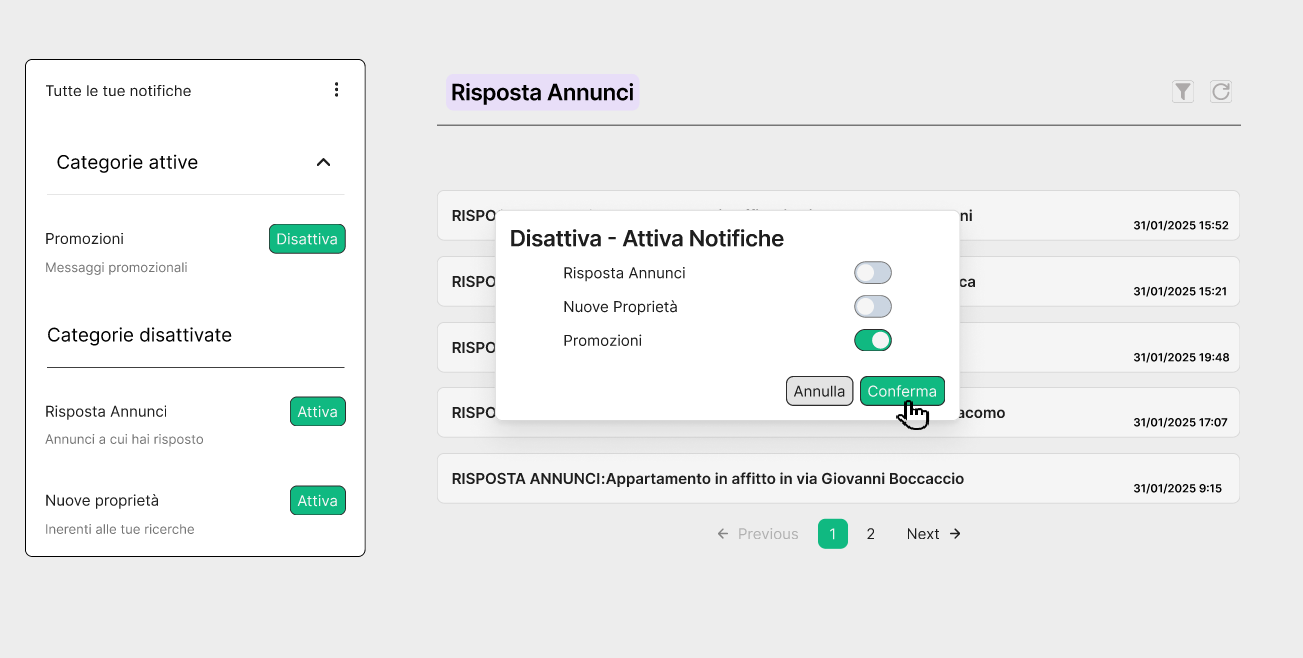
\includegraphics[width=0.7\textwidth]{Immagini/Mockup/notifiche/scenario principale/clickConferma.png} \\
                Cockburn: step 5
            \end{tabular}
        };

        \node (img5) [below=of img4] {
            \begin{tabular}{c}
                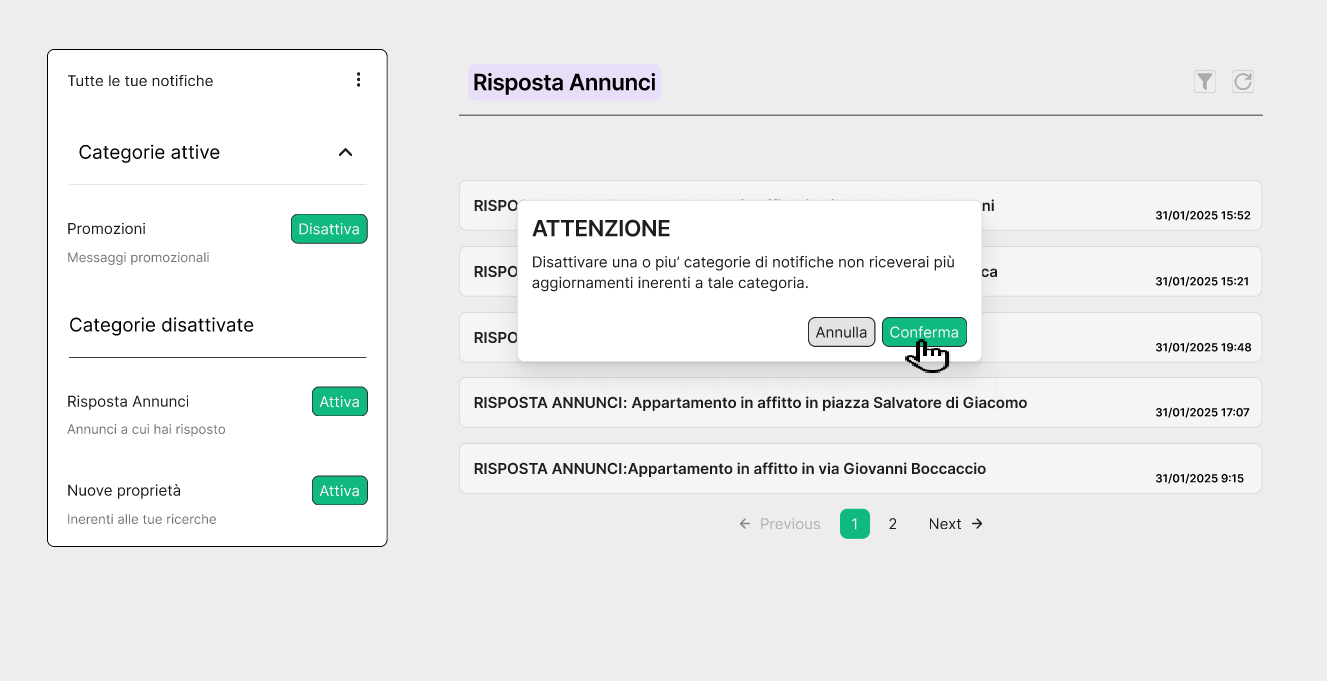
\includegraphics[width=0.7\textwidth]{Immagini/Mockup/notifiche/scenario principale/allerAvvisoDisattivazione.png} \\
                Cockburn: step 6/7
            \end{tabular}
        };

        \node (img6) [below=of img5] {
            \begin{tabular}{c}
                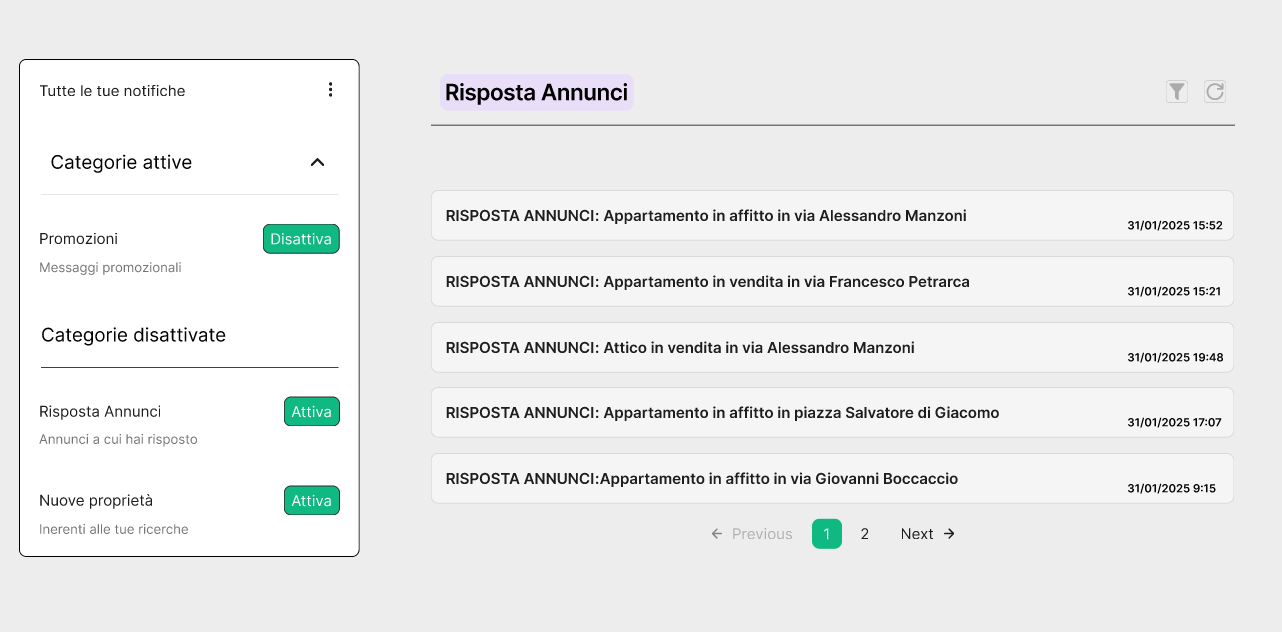
\includegraphics[width=0.7\textwidth]{Immagini/Mockup/notifiche/scenario principale/ScenarioPrincipaleCompletato.png} \\
                Conckburn: step 8/9/10
            \end{tabular}
        };
        
        % Disegna le frecce
        \draw[->, thick] (img4) -- (img5);
        \draw[->, thick] (img5) -- (img6);
        
    \end{tikzpicture}
    \caption{Parte 2 mockup: scenario principale della tabella di Cockburn del caso d'uso disattiva/attiva categoria notifica}
    \label{fig:mockup_scenario_principale_parte2_disattiva_notifiche}
\end{figure}